\chapter{System Design}
This chapter discusses the system design, analysing the various aspects of the project and purpose of each component such as the visualisation, the sorting algorithms, user authentication, the server, etc.

\section{Overview}
\begin{center}
    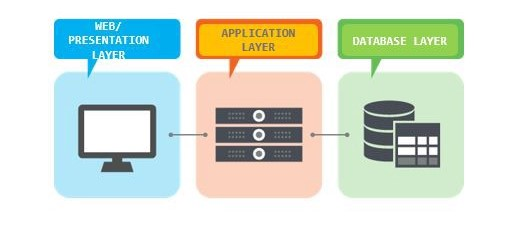
\includegraphics[width=8cm,height=3.3cm,keepaspectratio]{images/3tier}
\end{center}

This project utilises the multi-tier architecture (often referred to as n-tier architecture) platform. Multi-tier architecture or multilayered architecture is a client–server architecture in which presentation, application processing, and data management functions are physically separated. The most widespread use of multi-tier architecture is the three-tier architecture. This project consists of ... main components, all working together: The web application, which represents the presentation layer, allows users to visualise various sorting algorithms, register and login, upload and view past sorts from other users. The Flask server, which represents the logic tier, handles requests such as account registration and log in, and uploading and retrieving of sorts by users.

\begin{center}
    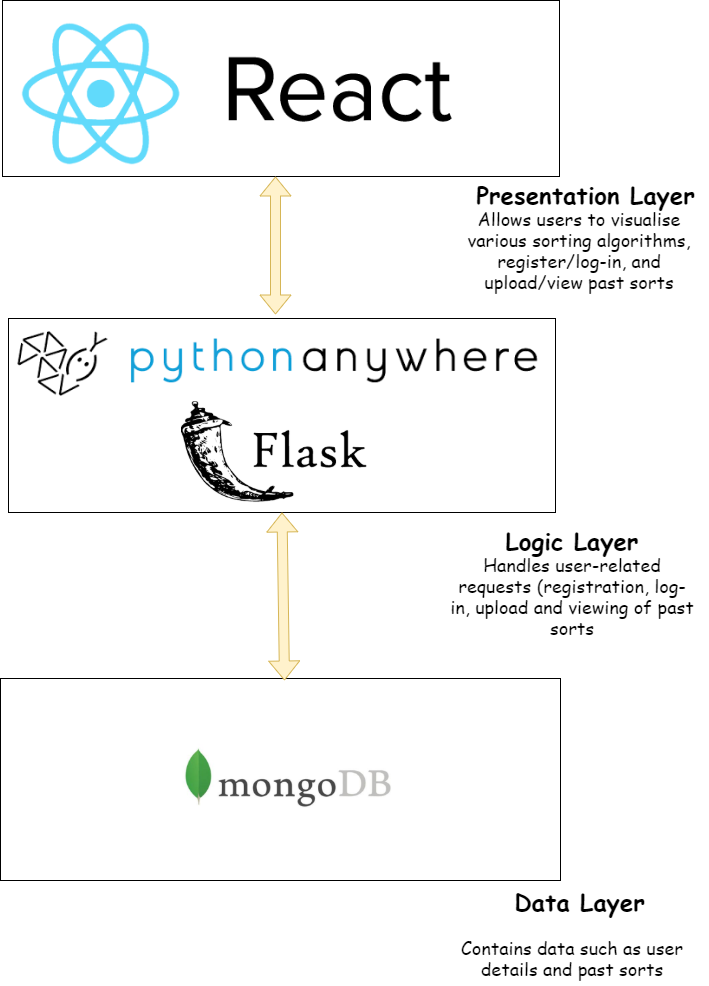
\includegraphics[width=15cm,height=12cm,keepaspectratio]{images/system_design}
\end{center}
\newpage

\section{Web Application}
The web application was designed and developed first as this is the main aspect of the project itself. The main objective of the web application was to allow a user to choose a sorting algorithm and be able to visualise it. Secondary objectives, which were developed at a later point, was to allow users to register and log in to an account, and have the ability to upload and view previous sorts. This was greatly aided by the decision to use ReactJS .... The web application consists of four main pages: 

\begin{itemize}
    \item \textbf{Sorting Page} - The sorting page, as shown in Figure \ref{fig:main_page}, is the main page of the application. Allows a user to choose one of several sorting algorithms to visualise, generate a random array of elements to sort, and specify their own dataset to sort.
    \item \textbf{Login Page} - The login page handles user authentication and will login a user to the application if that user exists within the database. The user will then be redirected to the sorting page, with new functionality available such as ...
    \item \textbf{Register Page} - The register page handles user authentication and will register a user with the application. The user will then be redirected to the login page, where they can then attempt to login.
    \item \textbf{Sorts Page} - The sorts page displays all previous sorts recorded and saved by past users.
\end{itemize}

\begin{figure}[!h]
    \centering
    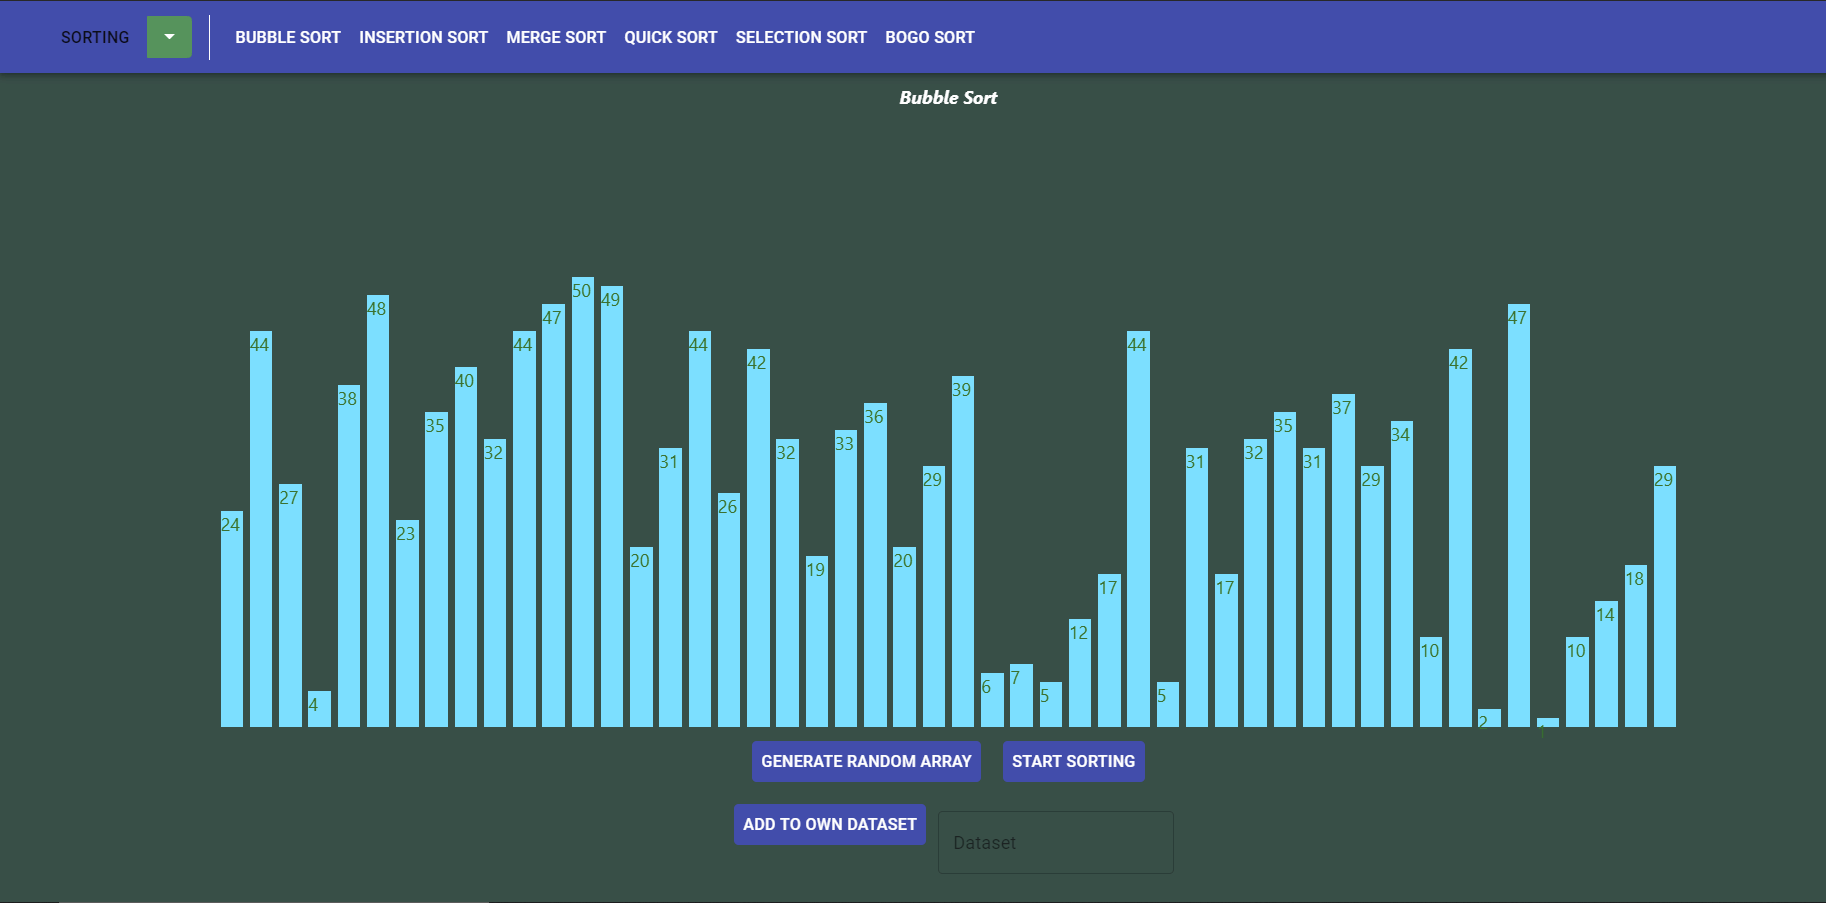
\includegraphics[scale=.4]{images/web_app_main}
    \label{fig:main_page}
\end{figure}

\subsection{Sorting}
\begin{center}
    \includegraphics[height=6.5cm,width=13cm]{images/sorting}
    \label{fig:main_page}
\end{center}

There are currently seven algorithms that can be visualised within the application. They are as follows:

\begin{itemize}
    \item Bubble Sort
    \item Heap Sort
    \item Insertion Sort
    \item Merge Sort
    \item Quick Sort
    \item Selection Sort
    \item Shell Sort
\end{itemize}

\subsubsection{Bubble Sort}
\begin{center}
    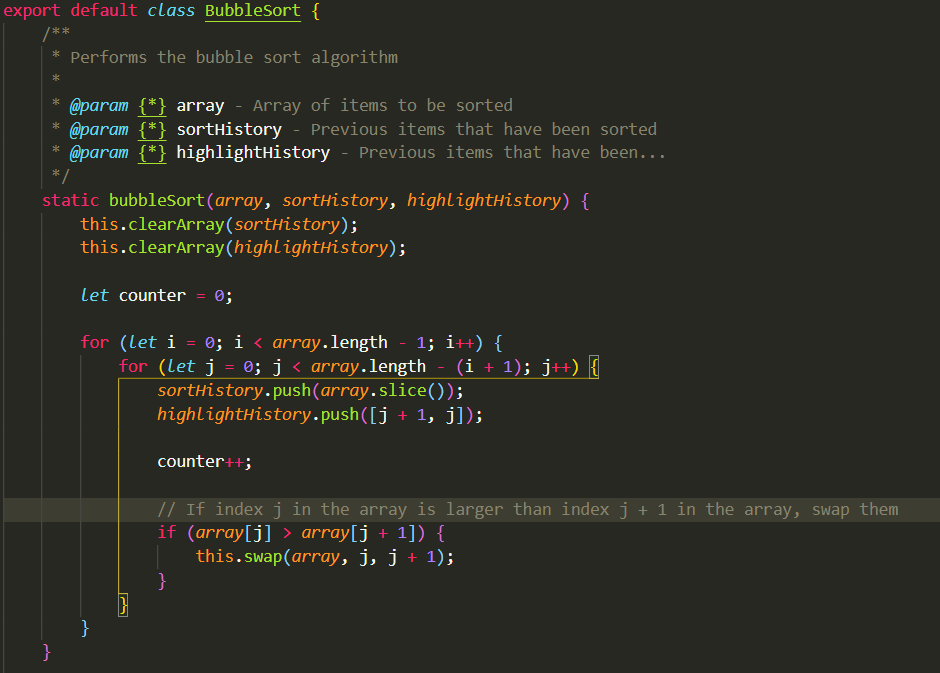
\includegraphics[width=12cm,height=15cm,keepaspectratio]{images/bubblesort}
\end{center}
Bubble sort, sometimes referred to as sinking sort, is a simple sorting algorithm that repeatedly steps through the list, compares adjacent elements and swaps them if they are in the wrong order. The pass through the list is repeated until the list is sorted. The algorithm, which is a comparison sort, is named for the way smaller or larger elements "bubble" to the top of the list.
\par
\bigskip
This simple algorithm performs poorly in real world use and is used primarily as an educational tool. More efficient algorithms such as Tim Sort, or Merge Sort are used by the sorting libraries built into popular programming languages such as Python and Java.

\subsubsection{Heap Sort}

\subsubsection{Insertion Sort}
\begin{center}
    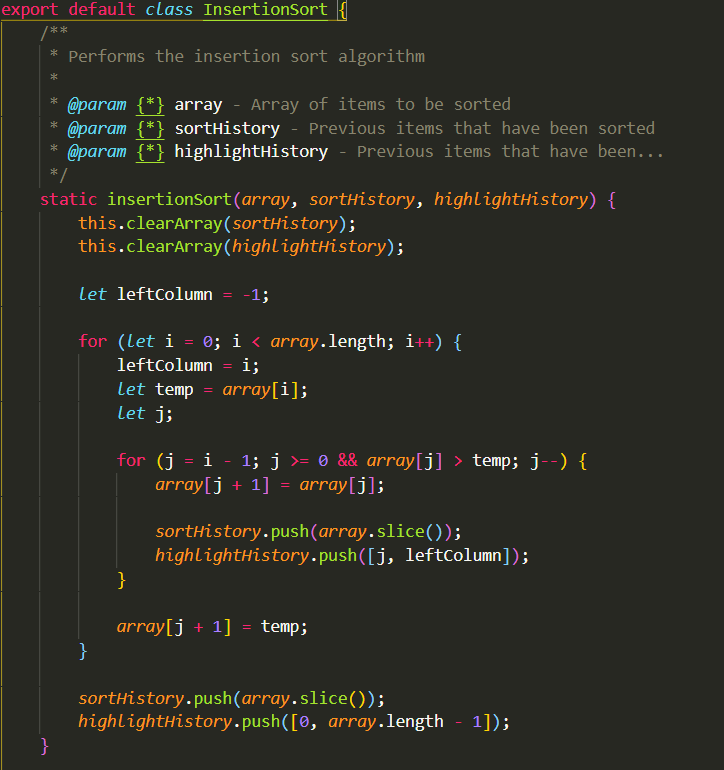
\includegraphics[width=12cm,height=15cm,keepaspectratio]{images/insertionsort}
\end{center}
Insertion sort is a simple sorting algorithm that builds the final sorted array (or list) one item at a time. It is much less efficient on large lists than more advanced algorithms such as Quick Sort, Heap Sort, or Merge Sort. However, insertion sort provides several advantages:

\begin{itemize}
    \item 
\end{itemize}

When people manually sort cards in a bridge hand, most use a method that is similar to insertion sort.

\subsubsection{Merge Sort}
\begin{center}
    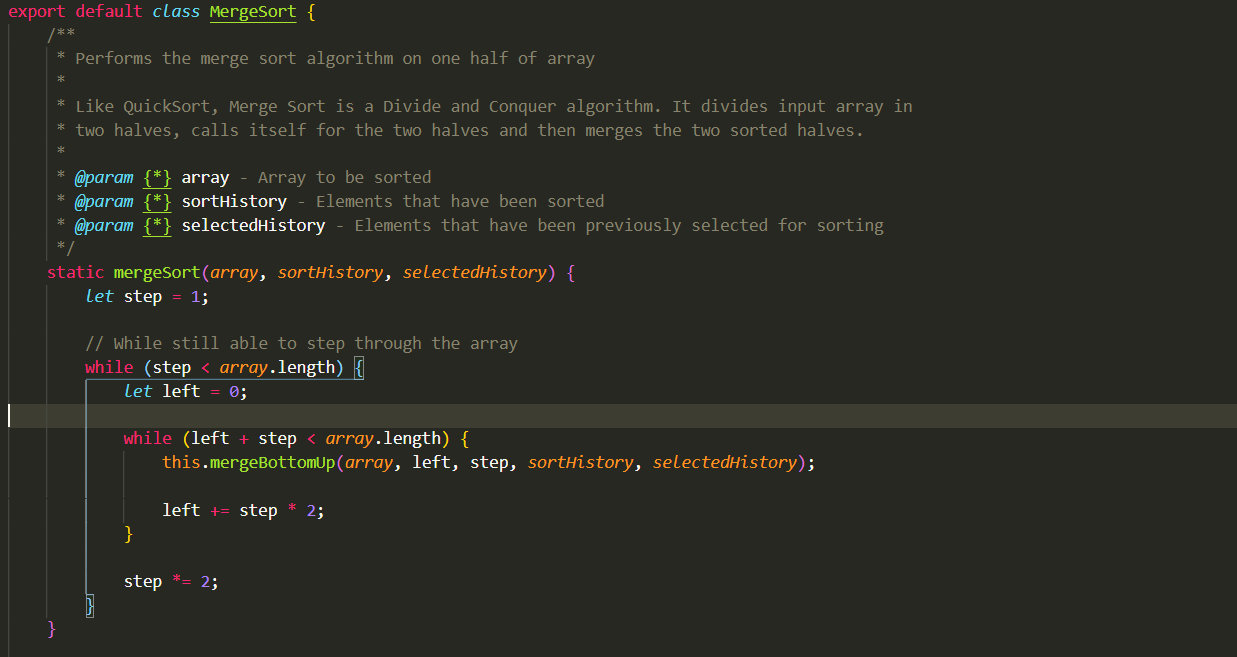
\includegraphics[width=12cm,height=15cm,keepaspectratio]{images/mergesort1}
    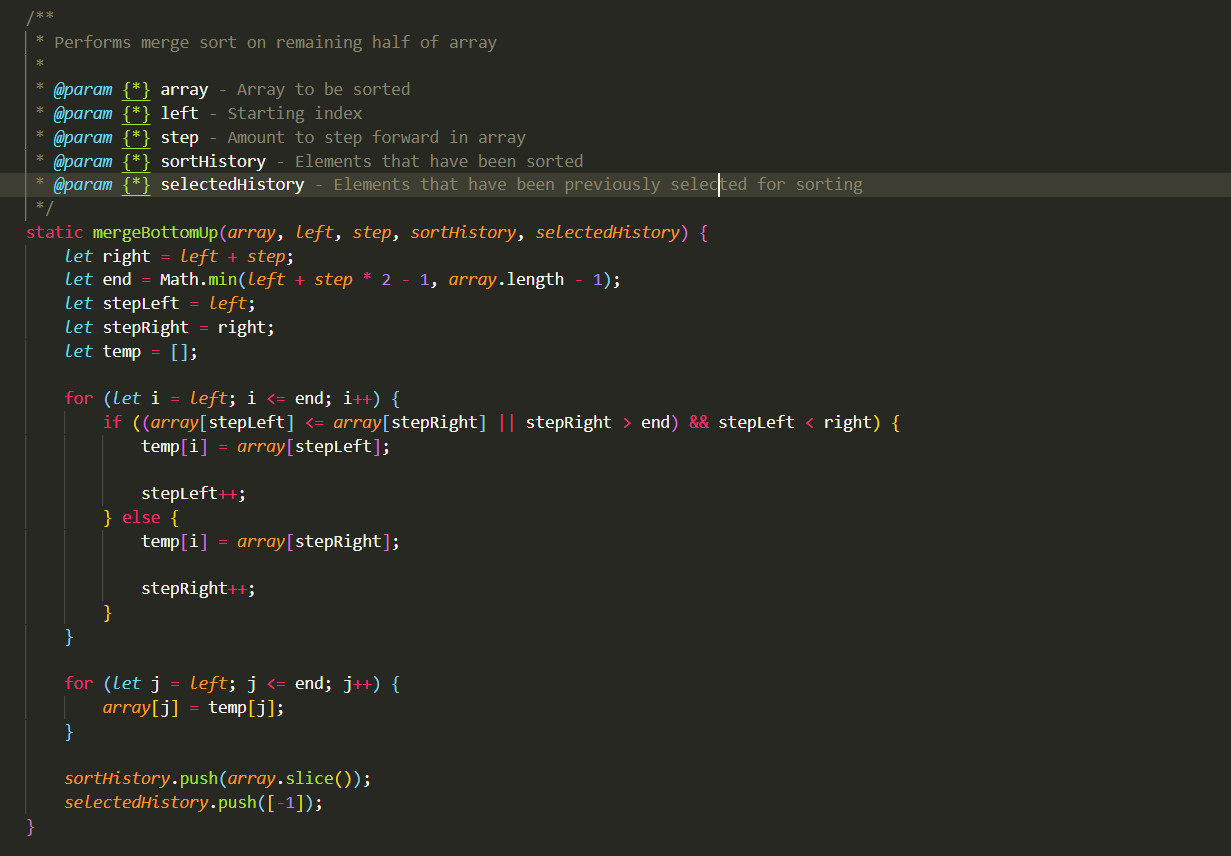
\includegraphics[width=12cm,height=15cm,keepaspectratio]{images/mergesort2}
\end{center}
In computer science, merge sort (also commonly spelled mergesort) is an efficient, general-purpose, comparison-based sorting algorithm. Most implementations produce a stable sort, which means that the order of equal elements is the same in the input and output. Merge sort is a divide and conquer algorithm that was invented by John von Neumann in 1945.[2] A detailed description and analysis of bottom-up mergesort appeared in a report by Goldstine and von Neumann as early as 1948

\subsubsection{Quick Sort}
\begin{center}
    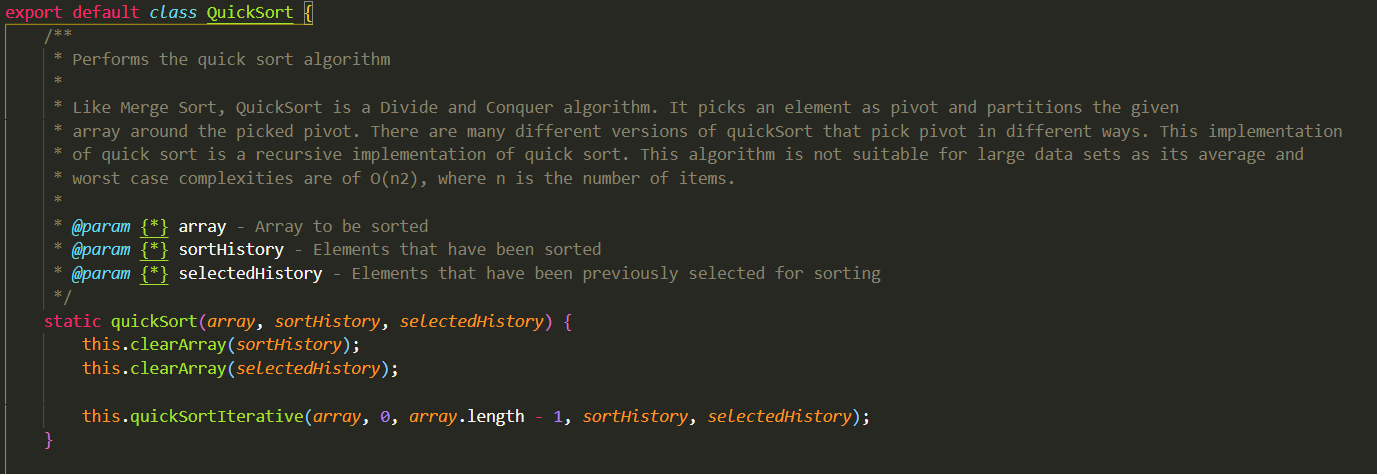
\includegraphics[width=15cm,height=15cm,keepaspectratio]{images/quicksort1}
    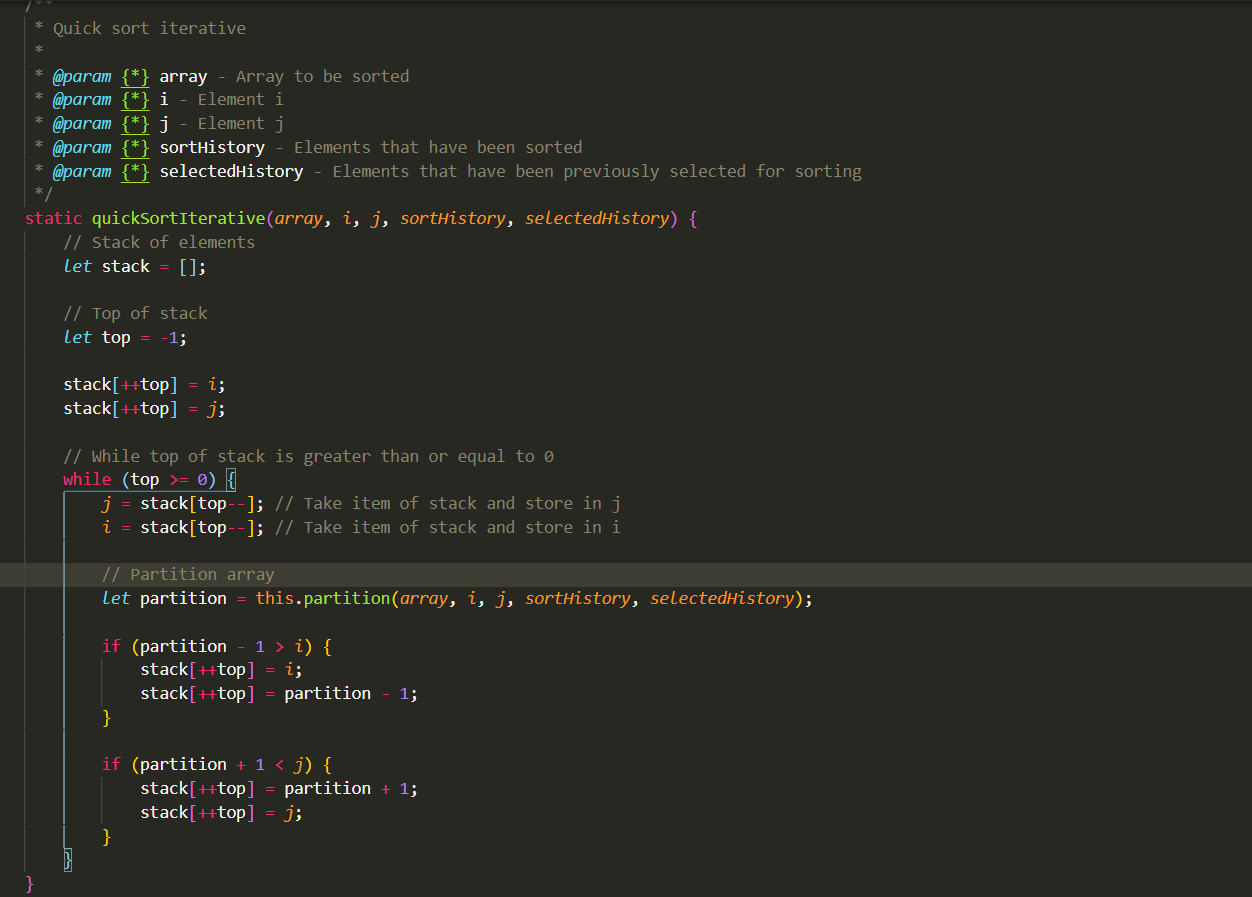
\includegraphics[width=15cm,height=15cm,keepaspectratio]{images/quicksort3}
    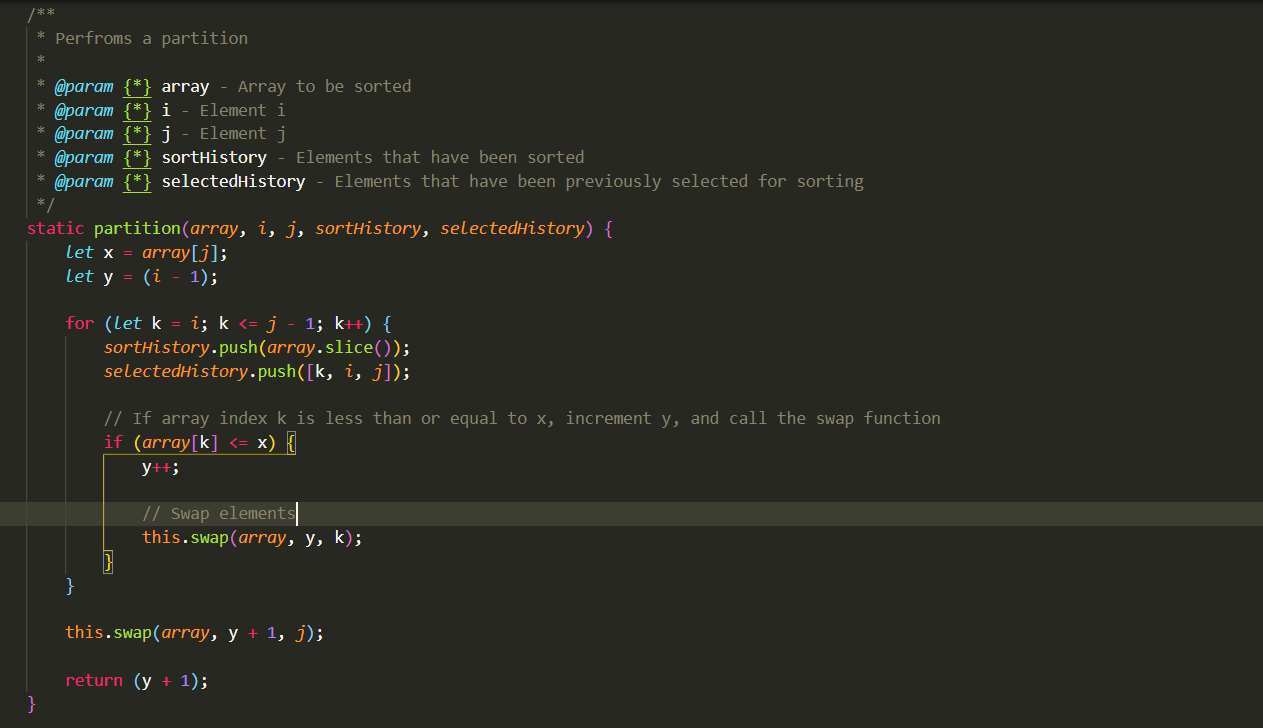
\includegraphics[width=15cm,height=15cm,keepaspectratio]{images/quicksort2}
\end{center}
Quicksort (sometimes called partition-exchange sort) is an efficient sorting algorithm. Developed by British computer scientist Tony Hoare in 1959[1] and published in 1961,[2] it is still a commonly used algorithm for sorting. When implemented well, it can be about two or three times faster than its main competitors, merge sort and heapsort.[3][contradictory]

Quicksort is a divide-and-conquer algorithm. It works by selecting a 'pivot' element from the array and partitioning the other elements into two sub-arrays, according to whether they are less than or greater than the pivot. The sub-arrays are then sorted recursively. This can be done in-place, requiring small additional amounts of memory to perform the sorting.

Quicksort is a comparison sort, meaning that it can sort items of any type for which a "less-than" relation (formally, a total order) is defined. Efficient implementations of Quicksort are not a stable sort, meaning that the relative order of equal sort items is not preserved.

Mathematical analysis of quicksort shows that, on average, the algorithm takes O(n log n) comparisons to sort n items. In the worst case, it makes O(n2) comparisons, though this behavior is rare.

\subsubsection{Selection Sort}
\begin{center}
    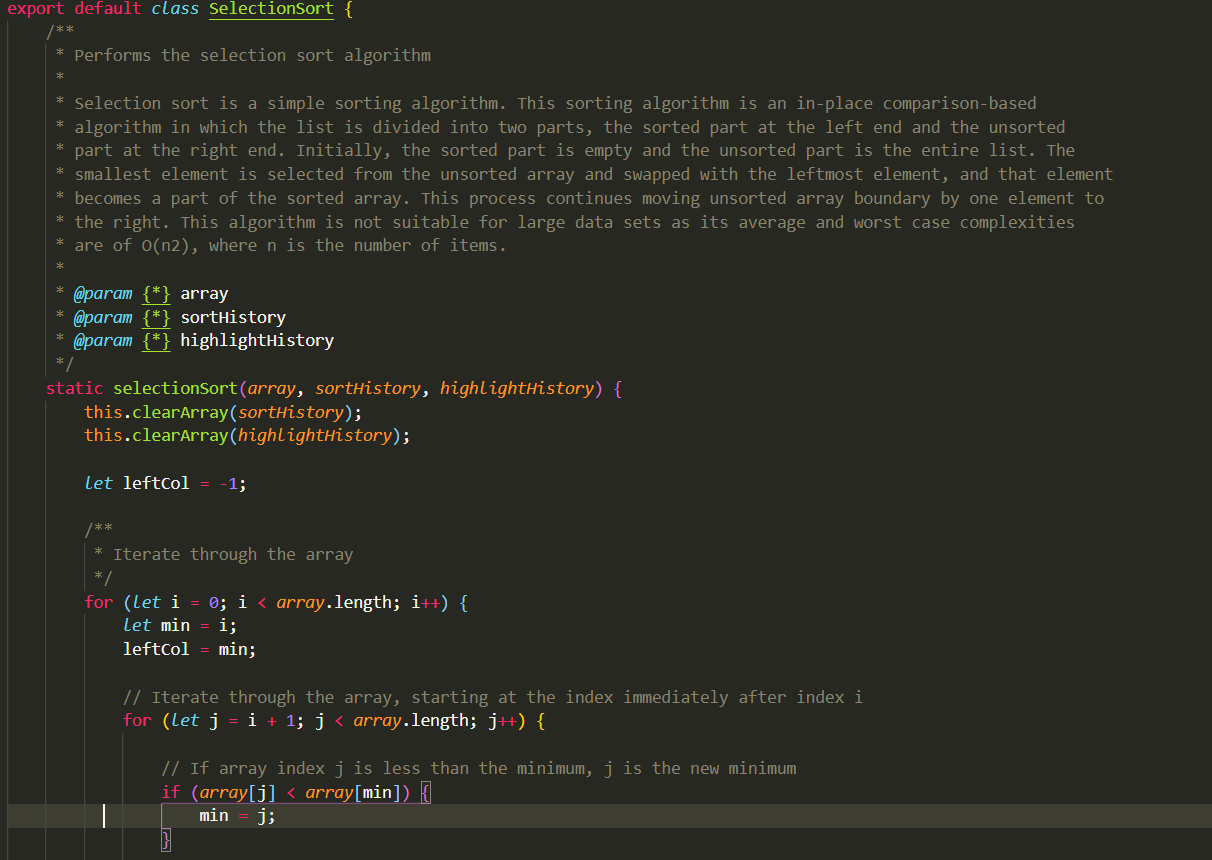
\includegraphics[width=12cm,height=15cm,keepaspectratio]{images/selectionsort1}
    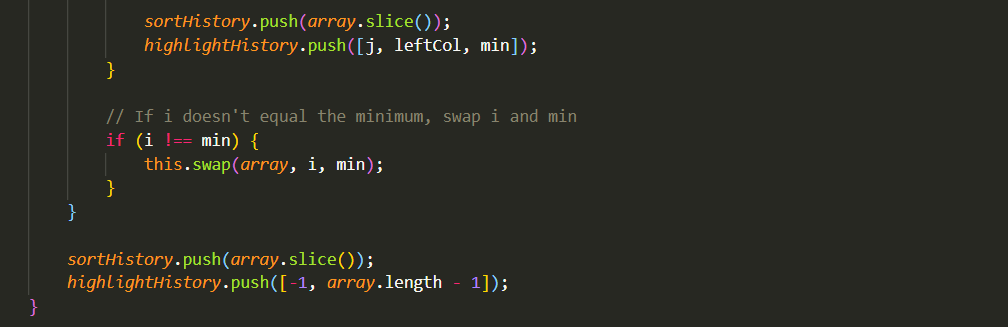
\includegraphics[width=12cm,height=15cm,keepaspectratio]{images/selectionsort2}
\end{center}
In computer science, selection sort is an in-place comparison sorting algorithm. It has an O(n2) time complexity, which makes it inefficient on large lists, and generally performs worse than the similar insertion sort. Selection sort is noted for its simplicity and has performance advantages over more complicated algorithms in certain situations, particularly where auxiliary memory is limited.
\par
\bigskip
The algorithm divides the input list into two parts: a sorted sublist of items which is built up from left to right at the front (left) of the list and a sublist of the remaining unsorted items that occupy the rest of the list. Initially, the sorted sublist is empty and the unsorted sublist is the entire input list. The algorithm proceeds by finding the smallest (or largest, depending on sorting order) element in the unsorted sublist, exchanging (swapping) it with the leftmost unsorted element (putting it in sorted order), and moving the sublist boundaries one element to the right.
\par
\bigskip
The time efficiency of selection sort is quadratic, so there are a number of sorting techniques which have better time complexity than selection sort. One thing which distinguishes selection sort from other sorting algorithms is that it makes the minimum possible number of swaps, n − 1 in the worst case.

\subsubsection{Shell Sort}

\subsection{Visualization}
\begin{center}
    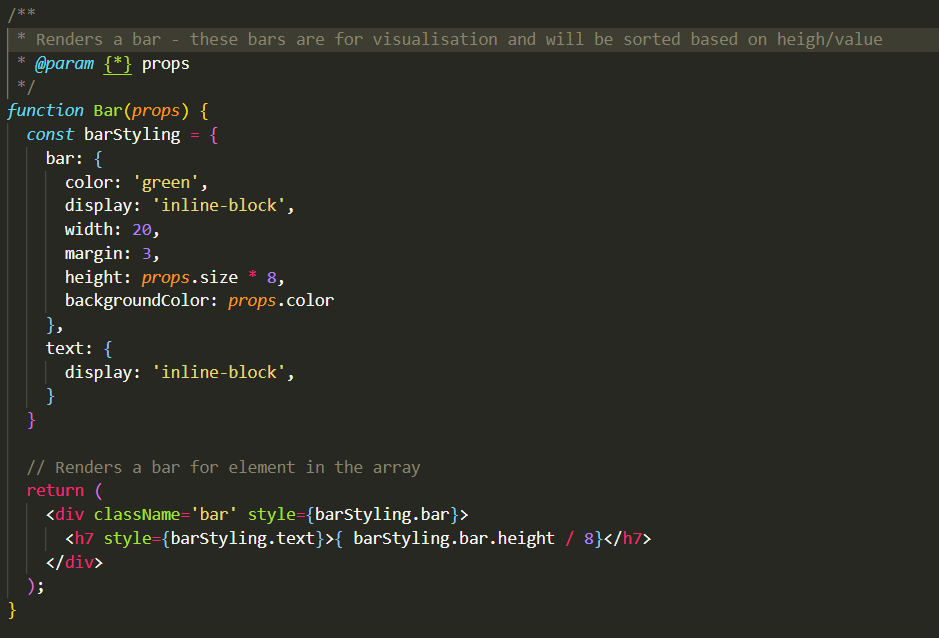
\includegraphics[height=6.5cm,width=10cm]{images/bar}
    \label{fig:main_page}
\end{center}

\section{Flask Server}
The Flask server, which is hosted on PythonAnywhere, is the middle-man of the entire application and allows the web application to communicate with the database. The server was developed and integrated into the web application secondly alongside the database. It handles requests, such as user login requests, user registration requests, uploading saved sorts, etc. made by the web application and performs the appropriate action. The database is then read and/or updated based on this. 

\begin{center}
    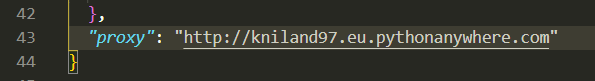
\includegraphics[width=15cm,height=10cm,keepaspectratio]{images/proxy}
    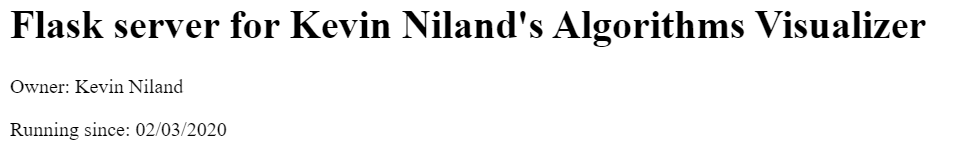
\includegraphics[width=15cm,height=10cm,keepaspectratio]{images/pa_kn}
\end{center}

\section{Database}
Fill out....